\section{Materiais e m�todos}\label{sec:materiaisMetodos}



De acordo com o que foi dito na Revis�o Liter�ria \ref{sec:revisaoLiteratura}, este trabalho segue arquitetura semelhante � utilizada em \cite{barra}.
Assim, dentro desta se��o ser� detalhada a Arquitetura Geral do Sistema \ref{subsec:arquitetura} e, em seguida, ser�o tratados os m�dulos componentes dessa arquitetura. Come�ando pelos dois grandes m�dulos constituintes dessa arquitetura: Navega��o \ref{subsec:navegacao} e Localiza��o \ref{subsec:localizacao}. A seguir, os componentes do M�dulo de Localiza��o ser�o detalhados: o Modelo de Din�mica \ref{subsec:modelodinamica} e os Modelos de Observa��o: Modelo de Observa��o dos Sonares \ref{subsec:modelosonares}, que se refere � nossa primeira abordagem; e Modelo Simples de Observa��o dos Sonares \ref{subsec:modeloSimplesSonar}, que se refere ao modelo final do trabalho e, por �ltimo, o Modelo de Observa��o da Vis�o \ref{subsec:modeloVisao}


\documentclass[a4paper,11pt]{article}
\usepackage{graphicx}
\usepackage[brazilian]{babel}
\usepackage[latin1]{inputenc}
\usepackage[T1]{fontenc}
\usepackage{amsmath, amsthm, amssymb, bm}
\usepackage[ruled,vlined,portugues]{algorithm2e}



\numberwithin{equation}{section}
\numberwithin{figure}{section}

\begin{document}



\subsection{Especifica��o}

O SAURON possui as seguintes especifica��es de Hardware e Software:

\begin{itemize}

\item{Plataforma rob� Pioneer 2DX, contendo:

\begin{itemize}
\item{Estrutura Mec�nica: motores e rodas;}
\item{Od�metro}
\item{Conjunto de 8 sonares;}
\end{itemize}}

\item{Notebook Embarcado;}
\item{C�mera de baixo custo;}
\item{Conex�o Serial-USB entre a plataforma-rob� e o notebook;}
\item{Conex�o USB entre c�mera e notebook ;}
\item{Software de Localiza��o;}
\item{Software de Navega��o;}


\item{Notebook }


\end{itemize}

\subsection{Arquitetura}\label{subsec:arquitetura}

A Arquitetura Geral do Sistema possui 5 grandes m�dulos: Interface Gr�fica, Navega��o, Localiza��o e Sensores e Motores, como pode ser observado na figura \ref{arquitetura:global}. O m�dulo de Navega��o pode ser dividido em Planejamento, Execu��o e Camada Reativa.
 
\begin{figure}[h]%
\begin{center}
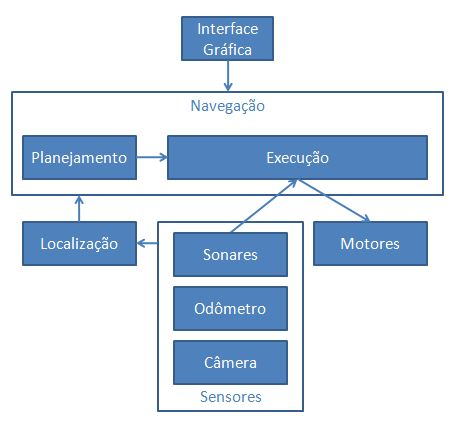
\includegraphics[width=.5\columnwidth]{imagens/arquiteturaGeral.jpg}
\caption{Arquitetura do sistema completo, descrevendo as interrela��es entre os m�dulos de localiza��o, navega��o e sensores}%
\label{arquitetura:global}%
\end{center}
\end{figure}

A interface gr�fica apresenta ao usu�rio os poss�veis destinos do rob� e repassa a escolha do usu�rio ao subm�dulo de planejamento, dentro do m�dulo de navega��o. A tarefa desse subm�dulo � calcular a melhor rota entre a postura atual e o destino. Como descrito na se��o \ref{subsec:navegacao}, utiliza-se um grafo de pontos chamados \textit{waypoints}. Cada waypoint � uma meta intermedi�ria, e um conjunto deles comp�e um caminho. O processo de locomo��o at� o pr�ximo \textit{waypoint} do caminho � coordenado pelo subm�dulo de execu��o, que dita � camada reativa a rota que dever� ser seguida, e monitora seu correto cumprimento. A camada reativa, por fim, � respons�vel por controlar os motores e monitorar as leituras dos sonares, de modo a detectar obst�culos din�micos e impedir colis�es.

A estimativa da postura (i.e, coordenadas $x$, $y$ e $\theta$) � realizada pelo m�dulo de localiza��o, que se vale dos dados dos sensores, al�m de seu conhecimento do ambiente. Neste caso, s�o fornecidos uma planta geom�trica e um mapa de marcos visuais. A arquitetura do m�dulo de localiza��o � descrita na se��o \ref{subsec:arqloc}.

Finalmente, o m�dulo de sensores � composto por sonares, od�metro e uma c�mera, que fornecem as informa��es necess�rias para o M�dulo de Localiza��o estimar sua postura (i.e, coordenadas $x$, $y$ e $\theta$). 
\section{Navega��o}\label{subsec:navegacao}

A arquitetura do m�dulo de navega��o est� representada na figura \ref{navegacao:arquitetura}, e possui os subm�dulos de planejamento intermapas, planejamento de rota e execu��o. Este m�dulo de navega��o foi totalmente desenvolvido pela equipe, caracterizando-se como uma das contribui��es deste trabalho.


\begin{figure}[h]%
\begin{center}
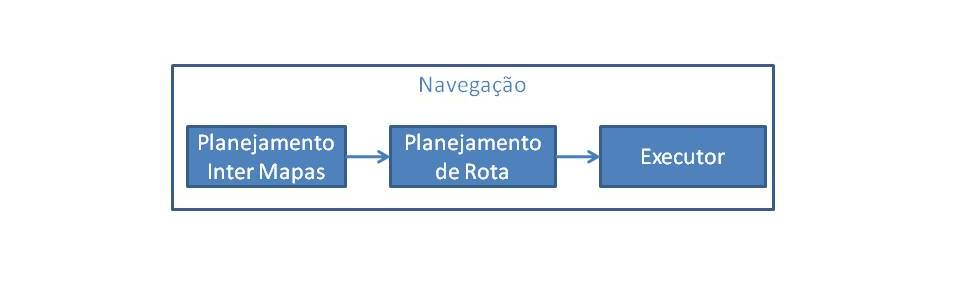
\includegraphics[width=.5\columnwidth]{imagens/arquiteturaNavegacao.jpg}
\caption{Arquitura do m�dulo de navega��o}%
\label{navegacao:arquitetura}%
\end{center}
\end{figure}

O objetivo do m�dulo de navega��o � guiar o SAURON at� destinos escolhidos por um usu�rio, dentro de um conjunto de mapas previamente informados. Al�m disso, o m�dulo deve trabalhar de modo a otimizar o resultado do m�dulo de localiza��o, essencial ao bom funcionamento do sistema. Para o m�dulo de localiza��o detalhado na se��o anterior, nota-se que a participa��o do od�metro prejudica consideravelmente a estimativa da postura durante a realiza��o de curvas, portanto, o m�dulo aqui descrito tem, como uma de suas prioridades: uma atua��o de forma a realizar poucas curvas.

Os mapas utilizados pelo SAURON foram marcados com alguns pontos, formando n�s de um grafo e permitindo a utiliza��o de algoritmos de busca em grafos para planejamento de rota.

\subsection{Planejamento de rota}
O m�dulo de navega��o usa o algoritmo de busca em grafo conhecido por A* (l�-se "A estrela") \cite{Korf85depth-firstiterative-deepening}. Ao adaptar esse problema � navega��o, os n�s do grafo passam a representar pontos em um mapa. Simplificadamente, pode-se dizer que o algoritmo parte de um n� inicial do seu grafo, a postura atual nesse caso, e come�a a visitar os n�s adjacentes, usando um crit�rio de custo para determina��o de qual n� deve ser visitado. O custo considerado � o custo de se locomover at� o n� adjacente somado ao custo de se locomover do n� adjacente at� o n� destino. 

Para possibilitar a busca em grafos, foram inseridos pontos de rota (ou \textit{waypoints}) no mapa utilizado pelo SAURON. Assim, os n�s do grafo utilizado pelo algoritmo s�o os \textit{waypoints} e os objetivos (ou \textit{goals}). Os \textit{goals} representam os pontos de interesse para os usu�rios (e.g., ``sala C2-50'', sala ``D1-30'' etc.) e j� existiam no mapa originalmente. Os \textit{waypoints} s�o pontos artificiais, criados para servir de rota para a navega��o.

Os \textit{waypoints} s�o colocados afastados das bordas do mapa e em pontos estrat�gicos escolhidos para permitir a realiza��o de curvas e facilitar a locomo��o a qualquer um dos objetivos.

Apesar do grafo de navega��o conter esses dois tipos de n�, apenas os \textit{waypoints} s�o usados para estabelecer a rota. O \textit{goal} s� servir� como n� final, ou seja, destino da navega��o. O n� inicial � um n� tempor�rio, inexistente no mapa, criado no in�cio da execu��o do algoritmo com as coordenadas atuais do rob�. 

Com a estrutura do grafo pronta, basta aplicar o algoritmo A* para obter a sua rota.

\subsubsection{N� tempor�rio e Controle de Retrocessos} 

Imprecis�es e incertezas s�o inerentes a problemas de localiza��o e navega��o rob�ticas. � improv�vel que, em um determinado instante, o rob� esteja exatamente sobre um \textit{goal} ou \textit{waypoint} do mapa -- mesmo logo ap�s ter completado o percurso at� um desses n�s. Desse modo, � necess�rio que, a cada itera��o do algoritmo de execu��o, o planejamento seja refeito a partir de um n� tempor�rio correspondente � posi��o atual. Naturalmente, esse n� tempor�rio precisa ser ligado a um \textit{waypoint}, para que um caminho possa ser planejado. Um algoritmo simples para encontrar esse \textit{waypoint} � escolher o mais pr�ximo ao n� tempor�rio. Essa ideia resulta, contudo, em um grave problema: muitas vezes, o n� mais pr�ximo da posi��o atual est� mais longe do destino final do que o pr�prio rob�. Navegar at� ele significa um retrocesso indesejado.

Para resolver esse problema, n�o � suficiente considerar dist�ncia como dist�ncia euclidiana. Algumas vezes, � necess�rio afastar-se um pouco (afastamento no sentido puro de dist�ncia euclidiana) do destino antes de poder alcan��-lo.  A figura \ref{navegacao:mapaObstaculo} ilustra essa situa��o. Para ir do ponto A ao ponto D, deve-se contornar a parede, passando por exemplo, pelo ponto B, que est� mais afastado do destino D do que o pr�prio A.

\begin{figure}[h]%
\begin{center}
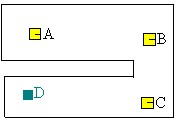
\includegraphics[width=.5\columnwidth]{imagens/mapaObstaculo.jpg}
\caption{Mapa que ilustra um problema comum a ser resolvido pela navega��o. Para navegar de A a D, � necess�rio se afastar do objetivo para depois alcan��-lo.}%
\label{navegacao:mapaObstaculo}%
\end{center}
\end{figure}

Deve-se, ent�o, considerar o custo de um n� at� o destino como sendo o custo da rota e n�o como a dist�ncia euclidiana entre esses dois pontos. Utilizando como exemplo a figura \ref{navegacao:mapaObstaculo}, o custo do n� B � menor que o custo do n� A.

� poss�vel resolver o problema de retrocessos com n�s tempor�rios. Descobre-se, para a posi��o atual, o n� alcan��vel, i.e., um n� naveg�vel em linha reta sem obst�culos que possua o menor custo at� o destino, $N�_{alcancavel}$. Escolhe-se como o \textit{waypoint} adjacente ao n� tempor�rio o \textit{waypoint} mais pr�ximo da posi��o atual que n�o esteja mais distante, metricamente, de $N�_{alcancavel}$ do que a posi��o atual do rob�.


\subsection{Execu��o e Controle de Rota} \label{sec:exec}

Assim que for definida uma rota de \textit{waypoints} at� o destino final, passa-se ao executor de rota, que opera da seguinte forma:

\begin{itemize}
	\item Realiza um giro at� ficar direcionado ao pr�ximo \textit{waypoint}.
	\item Desloca-se em linha reta at� alcan�ar o pr�ximo \textit{waypoint}.
\end{itemize} 

Essa estrat�gia de execu��o visa minimizar as incertezas em $\theta$, ao realizar o menor n�mero poss�vel de curvas. A motiva��o para isso � auxiliar o m�dulo de localiza��o, cujos sensores operam melhor sob movimento retil�neo.

Al�m disso, o subm�dulo executor tamb�m possui um comportamento de evitar colis�es, para que o rob� interrompa seu deslocamento caso detecte um obst�culo � frente.

Por fim, o subm�dulo executor possui um controle de rota, que determina quando o SAURON se afastou da rota prevista entre dois \textit{waypoints}. Quando isso ocorre, o rob� � parado e o planejamento recome�a.

\subsection{Navega��o Intermapas}

No intuito de possibilitar a navega��o em ambientes complexos e interligados, adicionou-se uma camada ao m�dulo de navega��o, para permitir a transi��o entre m�ltiplos mapas. Isso permite, por exemplo, subir uma rampa em dire��o a um outro andar de um pr�dio.

Para isso, carrega-se o sistema com todos os mapas dispon�veis e cria-se liga��es entre os mapas atrav�s de \textit{waypoints} especiais chamados portais.

Os portais s�o pontos comuns a dois mapas distintos e representam o mesmo ponto no mundo f�sico, por�m com coordenadas relativas diferentes em cada um dos mapas.

A camada intermapas � ent�o o ponto de entrada do m�dulo de navega��o, pois � respons�vel por gerenciar tamb�m a navega��o intramapa, utilizando as t�cnicas descritas acima. O algoritmo \ref{algo:intermapas} ilustra seu funcionamento. Nele, a refer�ncia \textbf{pathPlanner} indica o algoritmo de planejamento e navega��o intramapa.
   
 \begin{algorithm}
	\dontprintsemicolon
	
	\Entrada{destino}
	
	\Inicio{
		\Se{destino est� no mapa atual}{\ pathPlaner vai at� destino \;}
		\Senao{
			descobre pr�ximo mapa na rota de mapas \;
			acha portal em rela��o ao mapa atual \;
			\Se{pathPlanner chega em portal}
			{\ realiza troca de mapas \;
  		\ recome�a  \;}
  		\Senao{
			 erro \;
		}
	}
	}
	\caption{Algoritmo de navega��o entre m�ltiplos mapas}
		\label{algo:intermapas}
\end{algorithm}


A figura \ref{figura:navegacao} abaixo mostra o funcionamento global da navega��o. Os mapas s�o ligados atrav�s dos portais e, para cada mapa, � criada uma rota para o destino final dentro daquele mapa.


\begin{figure}[htbp]%
\begin{center}
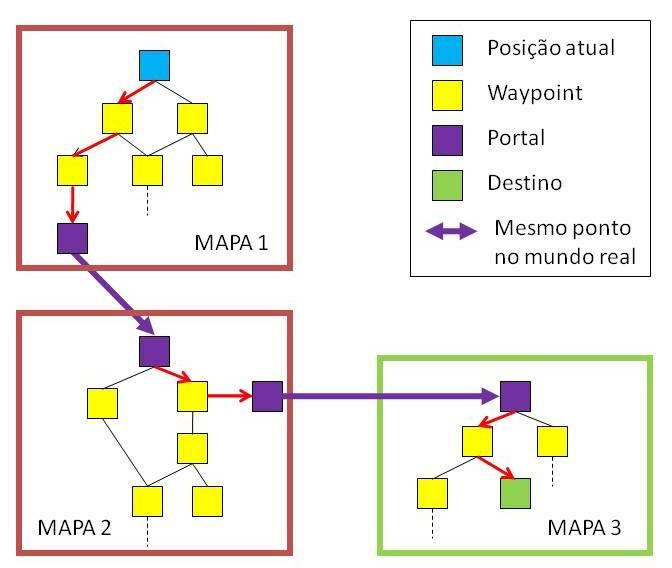
\includegraphics[width=.5\columnwidth]{imagens/navegacao.jpg}
\caption{Figura ilustrando funcionamento do m�dulo de navega��o.}%
\label{figura:navegacao}%
\end{center}
\end{figure}


Para determina��o da rota entre mapas utilizou-se um algoritmo de busca em profundidade aplicado ao grafo da rela��o entre os mapas (isto �, um grafo formado pelos portais). Como o n�mero de mapas ser� sempre pequeno, o tempo de busca � irris�rio e algoritmos mais complexos, como busca com profundidade limitada, n�o s�o necess�rios.
\section{Localiza��o}\label{subsec:arqloc}.

O sistema de localiza��o estima a postura do rob� a partir dos dados de seus sensores. O od�metro, sensor interno, � utilizado como uma medida da execu��o dos comandos de navega��o do SAURON, estando relacionado com um Modelo da Din�mica do Sistema. Os sensores externos t�m associados a si um modelo de observa��o, que descreve a rela��o da medida lida com o mundo real. Por exemplo, o modelo de observa��o do sonar associa uma leitura a uma parede no mapa. No restante deste texto, a palavra "sensor" indicar� um sensor externo.

O modelo de observa��o de cada sensor sabe qual � a observa��o esperada para uma dada postura do rob�, uma vez que conhece o mapa do ambiente. Uma diferen�a entre a observa��o esperada e a observa��o de fato recebida indica um erro na estimativa do sistema. Se os erros forem pequenos, podem ser consequ�ncia das varia��es naturais dos sensores f�sicos. Contudo, diferen�as grandes devem ser utilizadas para corrigir a postura. O pontocentral do algoritmo de localiza��o � exatamente este: a partir da diferen�a entre as observa��es esperadas e reais, corrigir a predi��o da postura.

Essas predi��es, que s�o corrigidas pelos modelos de observa��o dos sensores externos, s�o geradas pelo modelo de din�mica. O papel deste modelo � predizer a postura atual a partir da �ltima postura estimada do rob�, sabendo o quanto se andou nesse intervalo. Existem duas abordagens a esse problema. A primeira � utilizar os sinais de controle, como velocidade de cada roda, para prever o movimento do rob�. A segunda, utilizada neste trabalho, � obter as informa��es a partir do od�metro do rob�.

O uso de modelos de observa��o e de din�mica decorre da escolha pela utiliza��o de uma arquitetura baseada no uso do EKF. O EKF � um filtro matem�tico capaz de estimar o estado de um sistema n�o-linear a partir de predi��es do estado atual e de corre��es dessa predi��o. As equa��es para cada uma das etapas podem ser vistas na tabela \ref{table:kalman}, e s�o executadas na ordem da tabela. O EKF lineariza o sistema em sua borda a fim de que o filtro de Kalman comum possa ser utilizado com sucesso. Como o m�todo de lineariza��o utilizado no EKF � a expans�o de Taylor de primeira ordem, s�o geradas as matrizes $F$, jacobiano de $f(\textbf{x},\textbf{u})$, e $H$, jacobiano de $h(\textbf{x})$. 

\begin{table}[ht]
\centering
\begin{tabular}{ |c | c | }
\hline
\textbf{Predi��o} &  \textbf{Corre��o} \\ \hline
$\bar{\textbf{x}}_{t} = f(\textbf{x}_{t-1},\textbf{u}_{t-1})$ & $K_{t} = P_{t}^{-}H_{t}^{T}(H_{t}P_{t}^{-}H_{t}^{T}+R_{t})^{-1}$ \\ \hline
$P_{t}^{-} = F_{t-1}P_{t-1}^{+}F_{t-1}^{T} + Q_{t-1}$ & $\hat{\textbf{x}}_{t}^{+} = \hat{\textbf{x}}_{t}^{-} + K_{t}(\textbf{z}_{t}-h(\bar{\textbf{x}}_{t}^{-}))$ \\
& $P_{t}^{+} = (I - K_{t}H_{t})P_{t}^{-}$ \\ \hline
\end{tabular}
\label{table:kalman}
\caption{As equa��es principais do filtro de Kalman estendido (EKF).}
\end{table}

Os passos de funcionamento do m�dulo de localiza��o usando o EKF est� ilustrada na figura \ref{fig:dinamicaekf}. Inicialmente, tem-se uma postura estimada $\hat{\textbf{x}}_{t-1}$ que � usada para que o modelo de din�mica, atrav�s da leitura do od�metro, prediga uma nova postura $\bar{\textbf{x}_{t}}$. O sistema ent�o utiliza as medidas dos sensores para efetuar uma corre��o nessa predi��o, estimando a nova postura do rob�, $\hat{\textbf{x}_{t}}$, que � a sa�da do sistema. O processo se repete enquanto o m�dulo de localiza��o estiver ativo.

O �ltimo componente do sistema � o m�dulo de gerenciamento, que liga os demais componentes do sistema de localiza��o, iniciando os sensores e associando-os ao EKF.


\begin{figure}[ht]
	\centering
		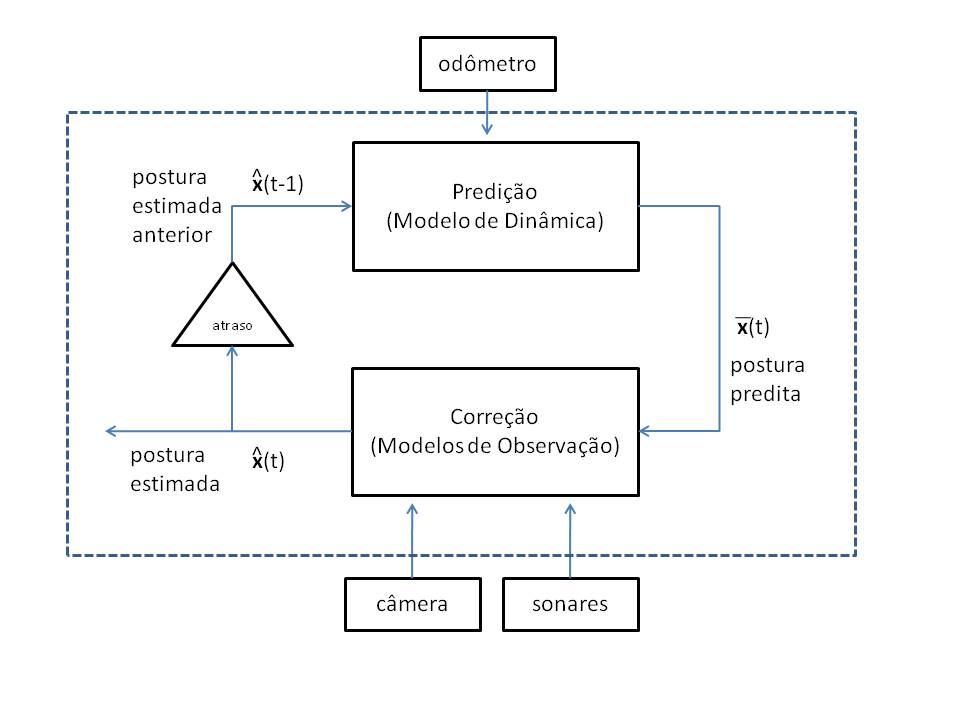
\includegraphics[width=.8\columnwidth]{imagens/dinamicaModuloLocalizacaoEkf.jpg}
	\caption{Din�mica do m�dulo de localiza��o, usando EKF.}
	\label{fig:dinamicaekf}
\end{figure}


A figura \ref{fig:arquiteturalocalizacao} ilustra a arquitetura do m�dulo de localiza��o. As informa��es retornadas pelos modelos dos sensores s�o a observa��o real ($\textbf{z}$), observa��o esperada ($\textbf{h}$), matriz de observa��o ($H$) -- que descreve como a observa��o depende dos componentes $x$, $y$ e $\theta$ da postura estimada -- e da covari�ncia($R$).


\begin{figure}[ht]
	\centering
		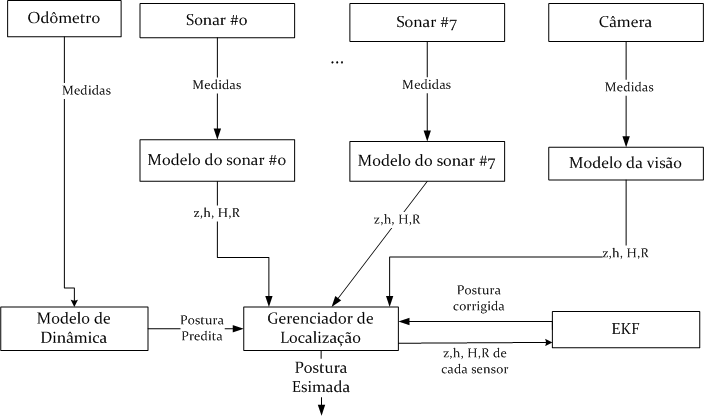
\includegraphics[width=.8\columnwidth]{imagens/arquiteturaModuloLocalizacao.png}
	\caption{Arquitetura do m�dulo de localiza��o}
	\label{fig:arquiteturalocalizacao}
\end{figure}

\subsection{Implementa��o}

Uma dificuldade em se implementar um sistema como o resumido acima � o controle do fluxo de execu��o. Para explicar o problema, pode-se observar o algoritmo \ref{algo:localizacao}, um esbo�o do funcionamento b�sico do m�dulo de localiza��o.

\begin{algorithm}
\dontprintsemicolon
\caption{Esbo�o do algoritmo do m�dulo de localiza��o}
\label{algo:localizacao}
\SetKw{recebe}{$\leftarrow$}
\SetKwBlock{RepitaSempre}{repita}{fim}
\SetKwData{ekf}{ekf}
\SetKwData{sensor}{sensor}
\SetKwData{dinamica}{din�mica}
\SetKwData{modeloObservacao}{modeloObservacao}
\SetKw{Em}{em}
\SetKwData{postura}{postura}
\RepitaSempre{
	\postura \recebe \ekf.predi��o(\dinamica.novaPredi��o()) \;
	\ParaCada{\modeloObservacao}{
		\Se{ \sensor.temMedidaNova()}{
			\postura \recebe \ekf.corre��o(\modeloObservacao.observacaoEsperada()) \;
		}
	}
	}\end{algorithm}

A implementa��o ing�nua desse algoritmo percorre os passos do pseudoc�digo sequencialmente, ou seja, itera pelo modelo de din�mica e por todos modelos de observa��o � procura daqueles que estejam prontos. A tabela \ref{tab:frequenciaSensores} mostra que os diferentes tempos de atualiza��o de cada modelo tornam essa abordagem invi�vel: na grande maioria das vezes, n�o haver� nenhum modelo de observa��o pronto, e a �nica estimativa ser� aquela fornecida pelo modelo de din�mica. Al�m disso, o la�o de processamento � executado o tempo todo, consumindo tempo de CPU e aumentando ainda mais o tempo de resposta dos modelos de observa��o.

\begin{table}[htbp]
	\centering
		\begin{tabular}{ | l | r | }
		\hline
		Modelo & Tempo entre atualiza��es (ms) \\ \hline
		Din�mica (Od�metro) & 5 \\ \hline
		Observa��o (Vis�o) & 25 \\ \hline
		Observa��o (Sonar) & 100 \\ \hline			
		\end{tabular}
	\caption{Frequ�ncia de atualiza��o dos modelos de din�mica e observa��o}
	\label{tab:frequenciaSensores}
\end{table}

A solu��o � transferir o controle do fluxo de execu��o de um m�dulo central para os modelos de observa��o. Quando um sensor receber novas medidas e for capaz de gerar uma observa��o esperada, ele chama o Gerenciador de Localiza��o, que ent�o invoca o EKF e computa a corre��o da estimativa. Esse processo � muito mais eficiente do que o \textit{polling}, pois n�o h� recursos desperdi�ados enquanto se espera inutilmente. A desvantagem do m�todo distribu�do � que um certo tempo deve ser perdido realizando a sincroniza��o de todas as \textit{threads} (para evitar, por exemplo, que dois sensores atualizem a estimativa ao mesmo tempo, corrompendo-a). A tabela \ref{tab:usoProcessador} relata os resultados obtidos, em termos do uso m�dio dos processadores, para cada abordagem, centralizada e distribu�da.

\begin{table}[htbp]
	\centering
		\begin{tabular}{ | l | r | }
		\hline
		Abordagem & Utiliza��o m�dia dos processadores \\ \hline
		Centralizada & 50\% \\ \hline
		Distribu�da & 11\% \\ \hline
		\end{tabular}
	\caption{Uso do processador nas duas abordagens de implementa��o (sistema com duas CPUs). O valor de 50\% significa uso completo de um dos n�cleos do computador port�til, ou seja, limita��o por processamento.}
	\label{tab:usoProcessador}
\end{table}